% !TeX root = main.tex

\section{FEDERATED SCHEDULING}
\label{sec: FEDERATED SCHEDULING}

\begin{frame}{セクションサマリ}
    \begin{itembox}[l]{\textbf{目的}}
        提案フェデレートスケジューリング, すなわち, 全てDAGがデッドラインに間に合うように各DAGに専用クラスタを割り当てる方法を提案
    \end{itembox}
    \begin{itembox}[l]{\textbf{流れ}}
        \setlength{\linewidth}{0.98\columnwidth}
        \begin{itemize}
            \item デッドラインを満たすことに関してDAGにとってプロセッサがどれほど「良い」かを直感的に示す, プロセッサバリューと呼ばれる概念を導入する
            \item 提案フェデレートスケジューリングアルゴリズムを説明
        \end{itemize}
    \end{itembox}
\end{frame}


\subsection{Processor Value}
\label{ssec: Processor Value}

\begin{frame}{事前準備1}
    「クラスタ $\mathcal{K}_y$ に属す $x$ 番目のプロセッサが, $G^j$に属すタスク $\tau_i$ に $s$ 番目の速度を提供するかどうか」を検出するブール型パラメーター $b_{s,x,y}^{i,j}$ を導入
    \begin{equation*}
        b_{s, x, y}^{i, j}= \begin{cases}\text { true } & \operatorname{ProcIndex}\left(O_{s, y}^{i, j}\right)=x \\ \text { false } & \text { otherwise }\end{cases}
    \end{equation*}
\end{frame}

\begin{frame}{事前準備2}
    プロセッサ $x$ をSpeed-Preferenceの $s$ 番目として持つ $G^j$内のタスクの数を検出する $cnt_{s,x,y}^j$ を導入
    \begin{equation*}
        c n t_{s, x, y}^j=\sum_{i=1}^{\mathcal{I}^j} b_{s, x, y}^{i, j}
    \end{equation*}
\end{frame}

\begin{frame}{プロセッサバリュー}
    \begin{definition}[$G^j$ に対するプロセッサ $x$ のプロセッサバリュー]
        \begin{figure}[tb]
            \centering
            \scalebox{0.8}{
                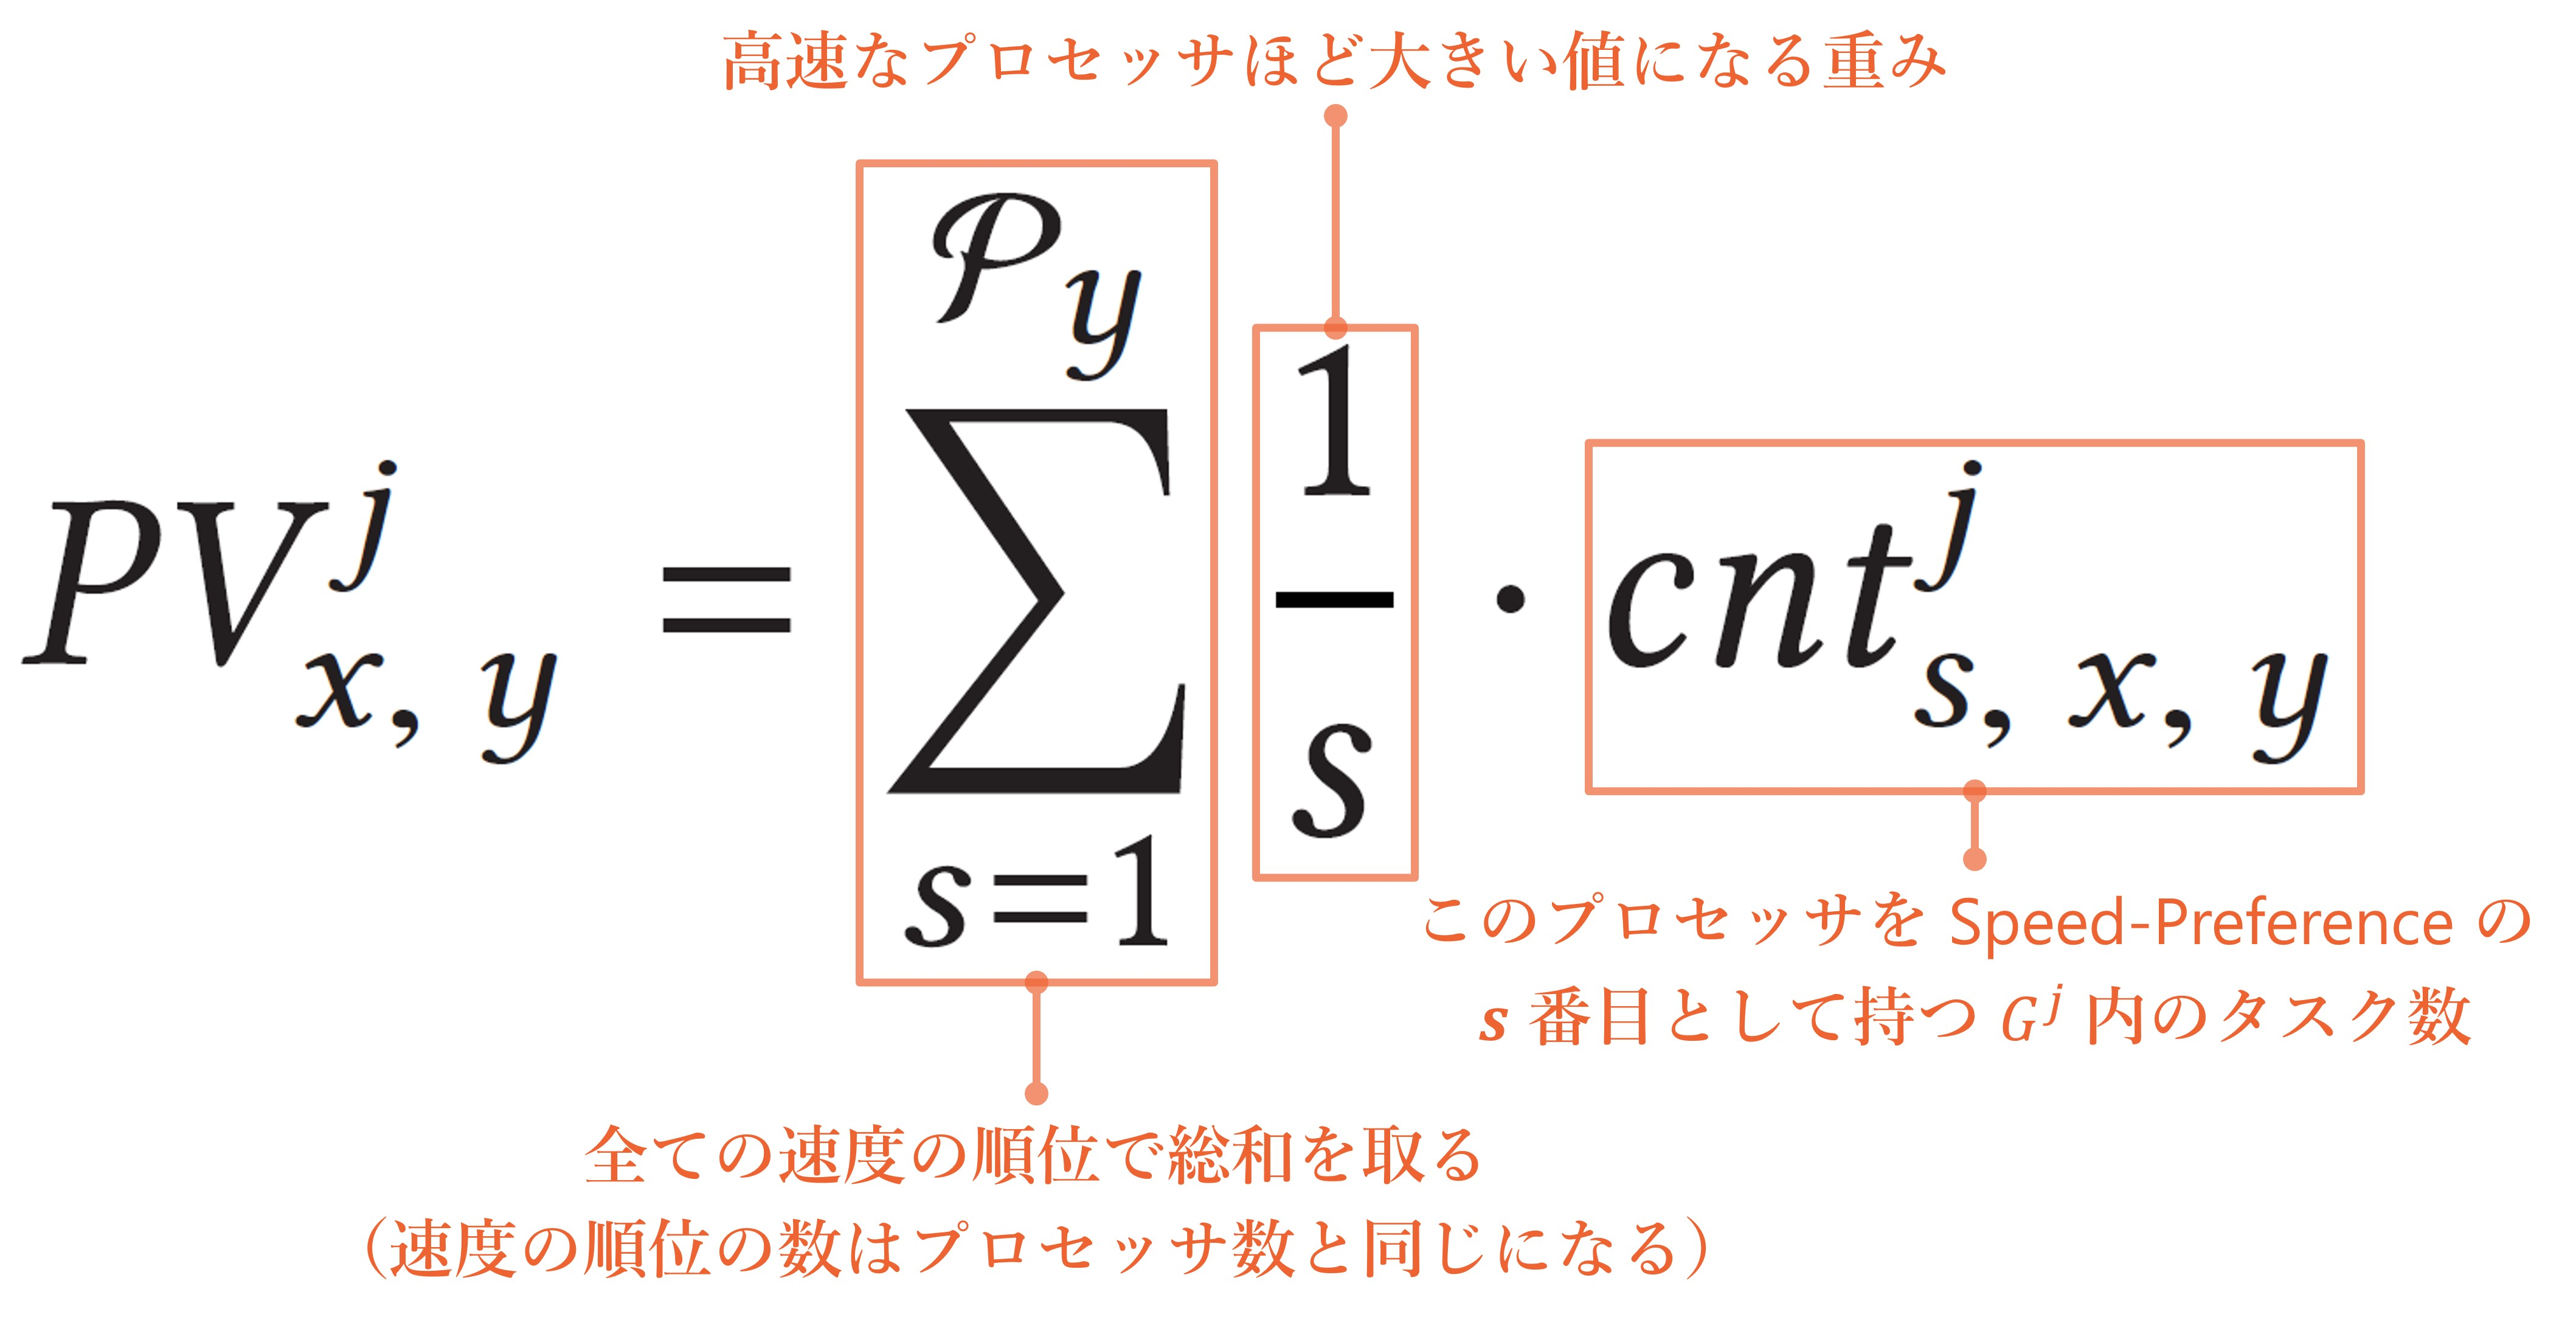
\includegraphics[width=\linewidth]{processor_value}
            }
        \end{figure}
    \end{definition}
\end{frame}

\begin{frame}{クラスタバリュー}
    プロセッサバリューをクラスタバリューに拡張する
    \begin{definition}[$G^j$ に対するクラスタ$\mathcal{K}_y$ のクラスタバリュー]
        \begin{figure}[tb]
            \centering
            \scalebox{0.6}{
                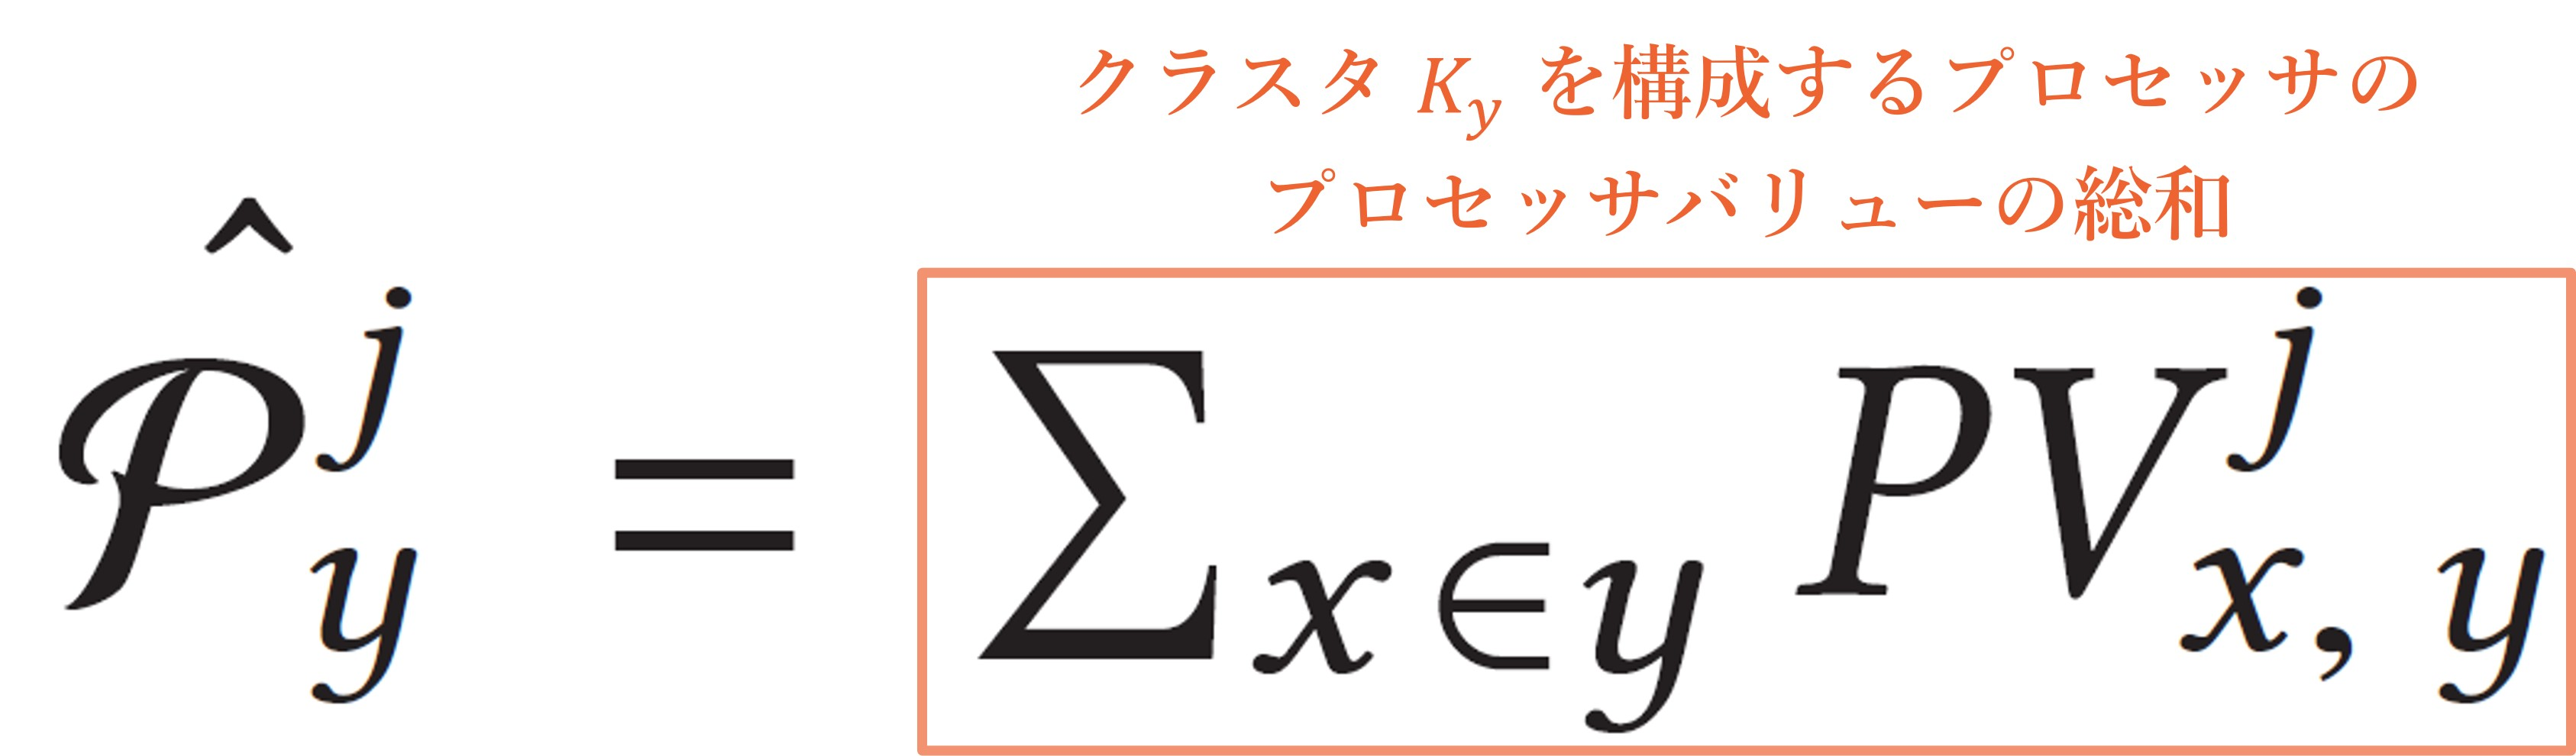
\includegraphics[width=\linewidth]{cluster_value}
            }
        \end{figure}
    \end{definition}
\end{frame}


\subsection{Description of the Algorithm}
\label{ssec: Description of the Algorithm}

\begin{frame}{提案フェデレートスケジューリング全体像}
    \fullimage{fed}
\end{frame}

\begin{frame}{提案フェデレートスケジューリング補足1}
    \fullimage{fed_sup1}
\end{frame}

\begin{frame}{提案フェデレートスケジューリング補足2}
    \fullimage{fed_sup2}
\end{frame}

\begin{frame}{提案フェデレートスケジューリング補足3}
    \fullimage{fed_sup3}
\end{frame}
